\chapter{Re-curation and rational enrichment of knowledge graphs in Biological Expression Language}
\label{ch:recuration}

\section*{Preface}

Following Chapters~\ref{ch:pybel} and~\ref{ch:belcommons} that laid the groundwork for handling and exploring knowledge graphs encoded in \ac{BEL}, the following publication describes the development and application of two workflows for 1) ensuring the quality of knowledge graphs encoded in \ac{BEL} and 2) enriching these knowledge graphs with semi-automated curation that leverages large-scale information extraction and natural language processing systems.
It presents an evaluation and comparison to previous semi-automated curation workflows using the metrics for curation overhead and efficiency described by Rodr\'{i}guez-Esteban~\cite{Rodriguez-Esteban2015}.

\vspace*{\fill}

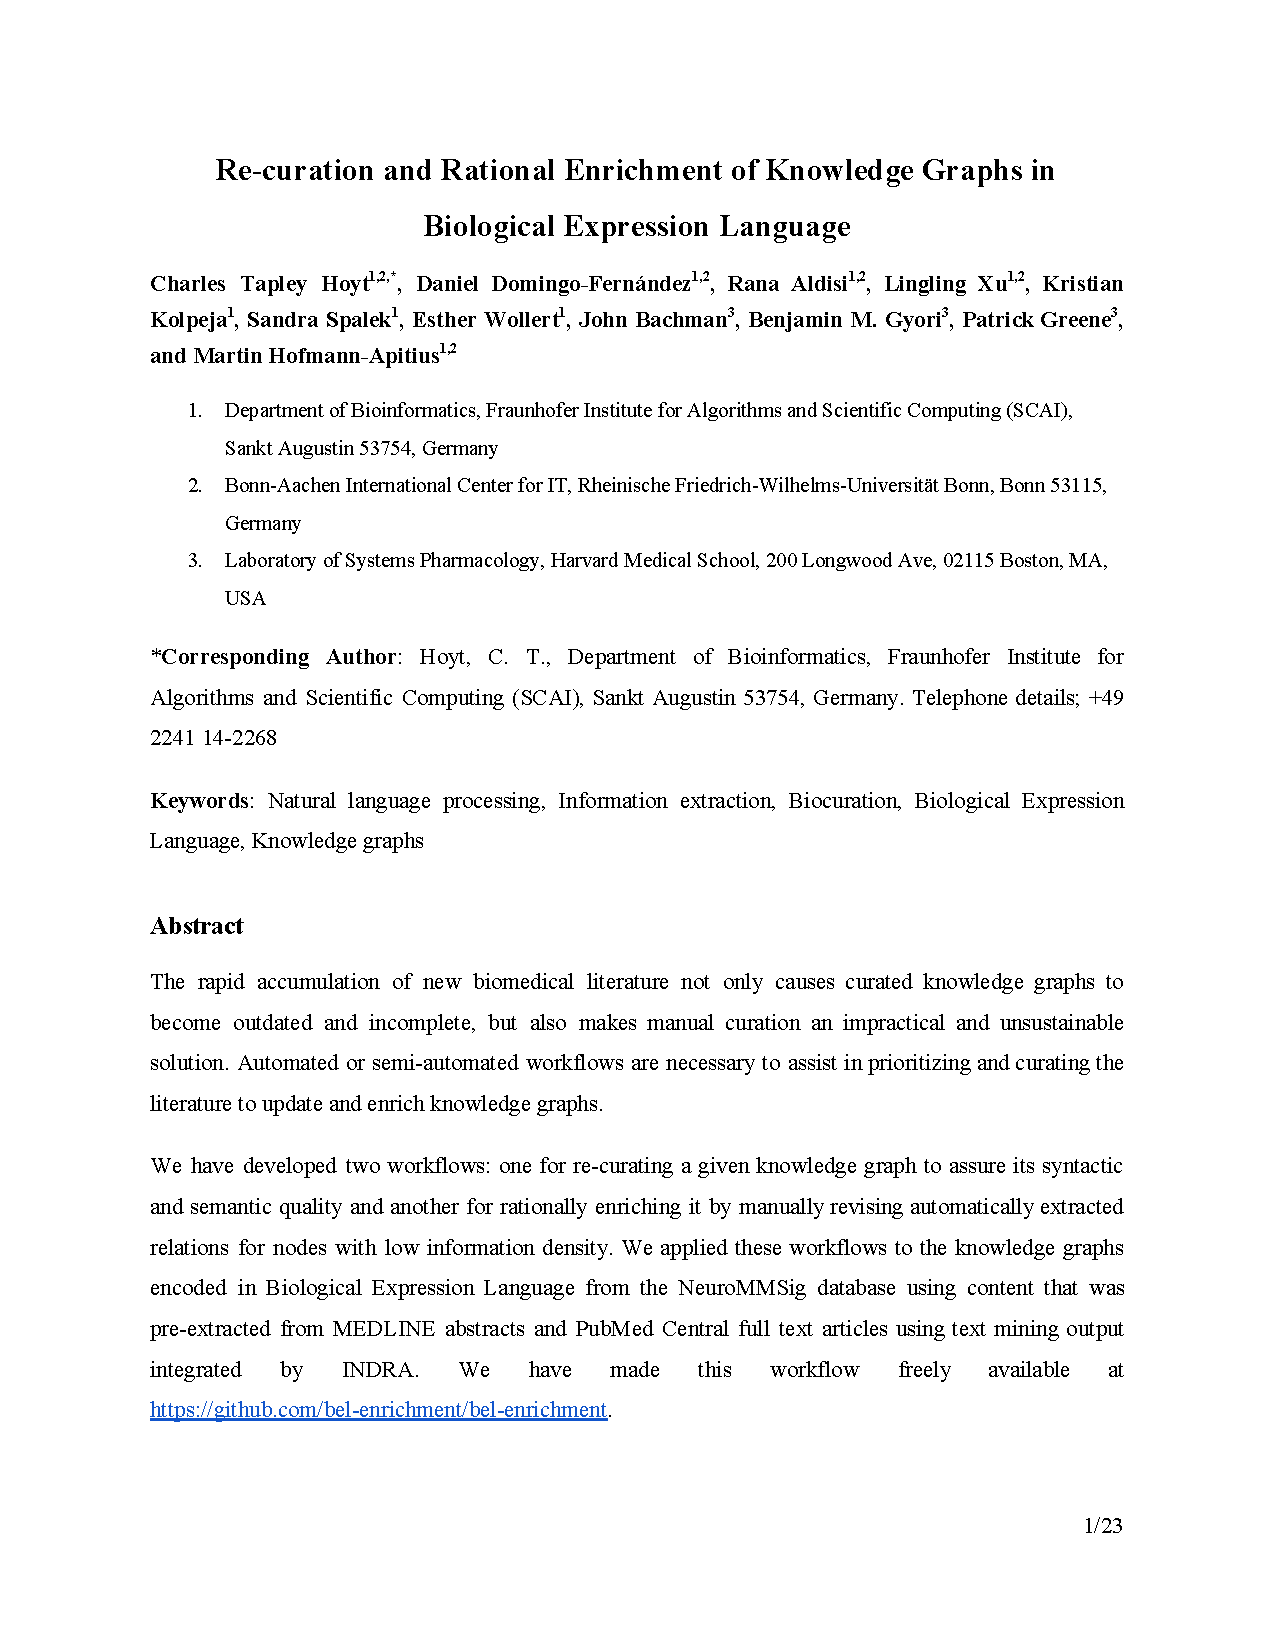
\includepdf[pages={-}]{articles/recuration.pdf}

\section*{Postface}

Continuing with the goals of developing the ecosystem around \ac{BEL} and PyBEL, the workflows and all resulting manually curated results from this publication have been made freely and openly available to the community.
The first workflow for quality control of \ac{BEL} promotes more sustainable curation practices through the usage of version control systems and continuous integration systems.
The second workflow allows for the usage of massively extracted content from unstructured text and automated enrichment of knowledge graphs, which further reduces this burden.
Ultimately, the usage of these workflows provided significant improvements over both manual curation and previously published state-of-the-art semi-automated curation systems.
These improvements manifested across all of the management, planning, and reading aspects of curation.
